\documentclass[a4paper, 11pt]{article}

% ==========================
% ENGLISH REPORT SETTINGS
% ==========================
\usepackage[english]{babel}
\usepackage{longtable}
\usepackage[table]{xcolor}
\usepackage{algorithmic}
% \usepackage{algorithm}

% ==========================
% UI AND TABLE SUPPORT
% ==========================

% geometry is the main layout package, so keep it near the top.
\usepackage[margin=2.5cm]{geometry} % Page margins

% \usepackage{a4wide} % Deprecated and conflicts with geometry
\usepackage{graphicx}
\usepackage{float}
\usepackage{array}    % Required by tabularx
\usepackage{multirow}
\usepackage{tabularx}
\usepackage{makecell}
\usepackage{booktabs}

% Font option
\renewcommand{\familydefault}{\sfdefault} % Use sans-serif as the default family.

% ==========================
% MATHEMATICS
% ==========================
\usepackage{amsmath, amssymb}

% ==========================
% FIGURES AND DIAGRAMS
% ==========================
\usepackage{subcaption}
\usepackage{tikz}
\usetikzlibrary{arrows,decorations,backgrounds,calc,positioning}
\usepackage{caption}
\captionsetup{font=footnotesize,skip=3pt}
\captionsetup[figure]{name=Figure}
\captionsetup[table]{name=Table}
% ==========================
% LISTS
% ==========================
\usepackage{enumitem}

% ==========================
% ALGORITHM
% ==========================
\usepackage[lined,boxed,commentsnumbered]{algorithm2e}

% ==========================
% FRAMES AND BOXES
% ==========================
\usepackage[framemethod=tikz]{mdframed}
\usepackage{tcolorbox}

% ==========================
% CODE LISTING
% ==========================
\usepackage{listings}
\definecolor{dkgreen}{rgb}{0,0.6,0}
\definecolor{gray}{rgb}{0.5,0.5,0.5}
\definecolor{mauve}{rgb}{0.58,0,0.82}

\lstset{
    frame=tb,
    language=matlab,
    basicstyle={\small\ttfamily},
    breaklines=true,
    keywordstyle=\color{blue},
    commentstyle=\color{dkgreen},
    stringstyle=\color{mauve},
    numbers=left,
    numbersep=4pt,
    numberstyle=\tiny\color{gray}
}

% ==========================
% HEADER & FOOTER
% ==========================
\usepackage{fancyhdr}
\usepackage{lastpage}
\setlength{\headheight}{40pt}

\pagestyle{fancy}

\fancyhead{} 
\fancyhead[L]{
 \begin{tabular}{rl}
    \begin{picture}(25,15)(0,0)
    \put(0,-8){\includegraphics[width=8mm]{graphics/logo_uit.png}}
   \end{picture}&
	\begin{tabular}{l}
		\textbf{\ttfamily Vietnam National University - Ho Chi Minh City}\\
  	\textbf{\ttfamily University of Information Technology}
	\end{tabular}
 \end{tabular}
}
\fancyhead[R]{}

\fancyfoot{}
\fancyfoot[L]{\scriptsize \ttfamily CS313 Project Report}
\fancyfoot[R]{\scriptsize \ttfamily Page \thepage/\pageref{LastPage}}

\renewcommand{\headrulewidth}{0.3pt}
\renewcommand{\footrulewidth}{0.3pt}

% ==========================
% TABLE OF CONTENTS DEPTH
% ==========================
\setcounter{secnumdepth}{4}
\setcounter{tocdepth}{3}

% ==========================
% SUBSUBSUBSECTION FORMAT
% ==========================
\makeatletter
\newcounter{subsubsubsection}[subsubsection]
\renewcommand\thesubsubsubsection{\thesubsubsection.\@alph\c@subsubsubsection}
\newcommand\subsubsubsection{\@startsection{subsubsubsection}{4}{\z@}
       {-3.25ex\@plus -1ex \@minus -.2ex}
       {1.5ex \@plus .2ex}
       {\normalfont\normalsize\bfseries}}
\newcommand*\l@subsubsubsection{\@dottedtocline{3}{10.0em}{4.1em}}
\makeatother

% ==========================
% HYPERLINK
% ==========================
\usepackage[colorlinks=true, linkcolor=black, citecolor=black, urlcolor=blue, breaklinks]{hyperref}

% ==========================
% TEMPLATE LAYOUT AND STYLES
% ==========================
\usepackage{style}
\usepackage{fontspec}
\setmainfont{TeX Gyre Termes}

\thesislayout


\begin{document}
\coverpage

\thispagestyle{empty}
%%%%%%%%%%%%%%%%%%%%%%%%%%%%%%%%%%%%%%%%%%%%%%
\newpage
\renewcommand{\contentsname}{Table of Contents}
\tableofcontents
%%%%%%%%%%%%%%%%%%%%%%%%%%%%%%%%%%%%%%%%%%%%%
\newpage
\small
\setlength{\parskip}{1pt}
\setlength{\parindent}{1em}
\setlength{\textfloatsep}{7pt plus 1pt minus 2pt}
\setlength{\floatsep}{6pt plus 1pt minus 2pt}
\setlength{\intextsep}{6pt plus 1pt minus 2pt}

\begin{center}
    {\Large\bfseries SaltySeq: Crop Stress Forecasting from Salinity Intrusion using Panel Time-Series Data and Sequential Pattern Mining}\\[0.35cm]
    {\normalsize CS313 - Data Mining Project Report}
\end{center}

\begin{abstract}
\noindent
This report presents SaltySeq, a data mining pipeline for forecasting crop stress caused by salinity intrusion at five monitoring stations in Ben Tre during 2015--2025. It constructs a daily panel dataset from satellite, weather, soil, and salinity signals, then derives rolling, lag, seasonal, and tendency features. To prevent temporal leakage, experiments use 2015--2022 for training, 2023--2025 for future holdout testing, and TimeSeriesSplit within the training set. The Optuna-tuned XGBoost model achieves test PR-AUC 0.9738, Recall 0.9387, and F2-score 0.9250. PrefixSpan provides interpretable environmental sequences, while GRU is explored as a high-recall but lower-precision deep learning extension.
\end{abstract}

\section{Introduction}

Salinity intrusion is a major agricultural risk in the Mekong Delta, especially in coastal provinces such as Ben Tre. Crop stress is not triggered by a single static salinity threshold. It is usually the cumulative result of salinity exposure, rainfall deficit, low soil moisture, surface heat, and vegetation decline over multiple days. Therefore, the problem is better formulated as a \textit{panel time-series classification} task: multiple monitoring stations, daily observations, heterogeneous data sources, and a binary stress label over time.

The objective of SaltySeq is to build a forecasting pipeline that is both methodologically rigorous and explainable enough for an academic demonstration: can multi-source daily environmental data forecast station-level crop stress while preserving temporal validity and avoiding leakage? The project makes three contributions: a daily panel dataset for five Ben Tre stations from 2015 to 2025 with 20,090 records and 70 merged columns; leakage-safe temporal evaluation using a future holdout set and imbalance-aware metrics; and a combined XGBoost--PrefixSpan design that provides strong performance with sequence-based explanations.

\section{Data Pipeline and Panel Construction}

The data pipeline follows the CRISP-DM philosophy: business understanding, data understanding, data preparation, modeling, evaluation, and deployment \cite{crispdm}. Instead of treating all rows as independent tabular samples, SaltySeq models each station as a time series inside a shared panel.

\begin{figure}[!htbp]
    \centering
    \begin{tikzpicture}[
        node distance=0.75cm,
        box/.style={draw, rounded corners, align=center, minimum height=0.85cm, text width=2.45cm, fill=blue!5},
        arrow/.style={->, thick}
    ]
        \node[box] (src) {Multi-source data\\GEE, Open-Meteo, salinity};
        \node[box, right=of src] (panel) {Daily panel\\5 stations, 2015--2025};
        \node[box, right=of panel] (feat) {Feature engineering\\rolling, lag, tendency};
        \node[box, right=of feat] (model) {XGBoost + PrefixSpan\\evaluation};
        \node[box, right=of model] (demo) {FastAPI demo\\map, gauge, history};
        \draw[arrow] (src) -- (panel);
        \draw[arrow] (panel) -- (feat);
        \draw[arrow] (feat) -- (model);
        \draw[arrow] (model) -- (demo);
    \end{tikzpicture}
    \caption{Overall pipeline: multi-source ingestion, daily panel construction, feature engineering, model training, and demo deployment.}
    \label{fig:pipeline}
\end{figure}

\subsection{Multi-source data ingestion}

The dataset is built from four main groups of inputs:

\begin{itemize}[leftmargin=1.2em, itemsep=1pt]
    \item \textbf{Monitoring locations}: five stations in Ben Tre, including Ba Tri, Binh Dai, Chau Thanh, Giong Trom, and Thanh Phu. Each station includes latitude, longitude, and distance to the estuary.
    \item \textbf{Satellite observations}: NDVI from Sentinel-2, Landsat 8/9, and MODIS; LST from Landsat through Google Earth Engine \cite{gorelick2017gee}. NDVI reflects vegetation health, while LST captures thermal stress.
    \item \textbf{Weather and soil}: temperature, precipitation, ET0, radiation, wind, surface/deep soil moisture, and soil temperature from the Open-Meteo Historical Weather API \cite{openmeteo}.
    \item \textbf{Salinity}: Copernicus Marine data is preferred when available \cite{copernicusmarine}; otherwise, the pipeline uses a salinity proxy based on seasonality, 7-day rainfall, ET0, estuary distance, and station-stable noise.
\end{itemize}

\subsection{Daily panel construction and provenance control}

After ingestion, all sources are aligned to the same key: \texttt{(location\_id, date)}. The pipeline creates a complete daily grid for each station, then merges satellite, weather, soil, and salinity variables by date. This design preserves station-specific temporal sequences while allowing the model to learn spatial differences through \texttt{lat}, \texttt{lon}, and \texttt{distance\_to\_estuary\_km}.

An important part of the pipeline is provenance tracking. Columns such as \texttt{ndvi\_source}, \texttt{ndvi\_interp\_method}, \texttt{ndvi\_is\_observed}, \texttt{ndvi\_gap\_days}, and \texttt{salinity\_source} distinguish direct observations, interpolated values, and proxy-generated signals. Because satellite observations are often missing due to cloud cover and revisit cycles, provenance metadata makes the dataset more transparent and supports interpolation-bias analysis during EDA.

The final merged dataset is stored as \texttt{merged\_final.csv} with 20,090 rows, corresponding to 5 stations $\times$ 4,018 days from 2015-01-01 to 2025-12-31. The positive stress-event rate is 10.8\%, indicating a clearly imbalanced classification problem.

\begin{table}[!htbp]
\centering
\caption{Summary of the merged panel dataset}
\label{tab:data-summary}
\small
\begin{tabularx}{0.95\linewidth}{lX}
\toprule
\textbf{Attribute} & \textbf{Value} \\
\midrule
Spatial coverage & 5 monitoring stations in Ben Tre \\
Temporal coverage & 2015-01-01 to 2025-12-31 \\
Records & 20,090 rows \\
Merged columns & 70 columns \\
Prediction label & $\texttt{is\_stress\_event} \in \{0,1\}$ \\
Positive rate & 2,171 / 20,090 = 10.8\% \\
Train / Test & 2015--2022 / 2023--2025 \\
\bottomrule
\end{tabularx}
\end{table}

\section{Data Understanding and EDA}

EDA is designed to answer three questions: whether stress is seasonal, how coastal stations differ from inland stations, and whether satellite-derived vegetation signals may be biased by interpolation. The main views include the NDVI z-score timeline, the five-station NDVI panel, source coverage, annual stress rate, and interpolation-bias analysis. This step prevents the model from being misread as a simple salinity-threshold alarm.

\begin{figure}[!htbp]
    \centering
    \begin{subfigure}{0.88\linewidth}
        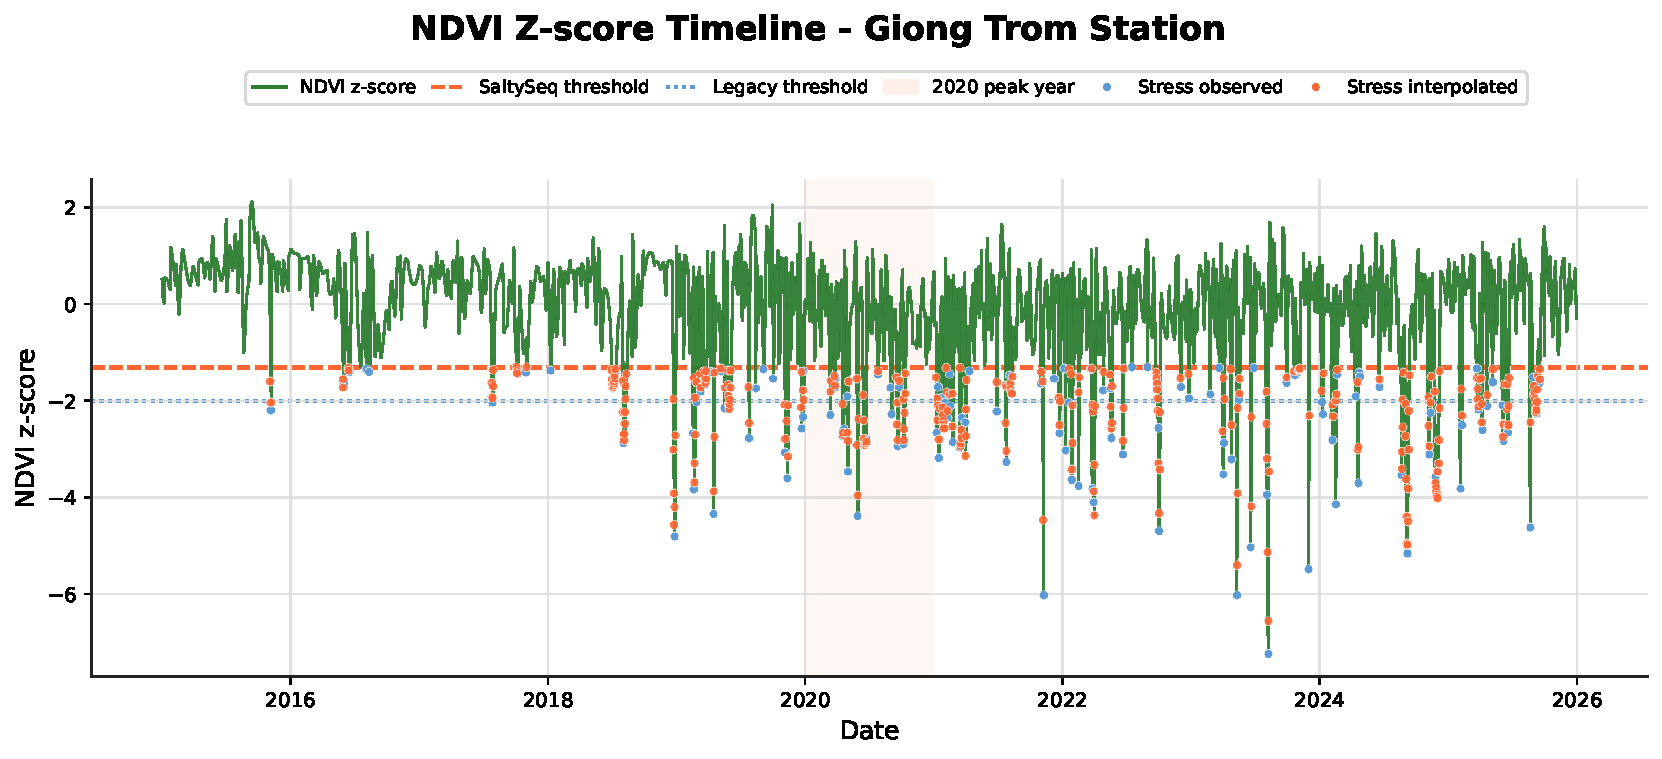
\includegraphics[width=\linewidth]{report_figures/fig1_ndvi_zscore_timeline.pdf}
        \caption{NDVI z-score and stress events}
    \end{subfigure}
    \vspace{0.05cm}
    \begin{subfigure}{0.88\linewidth}
        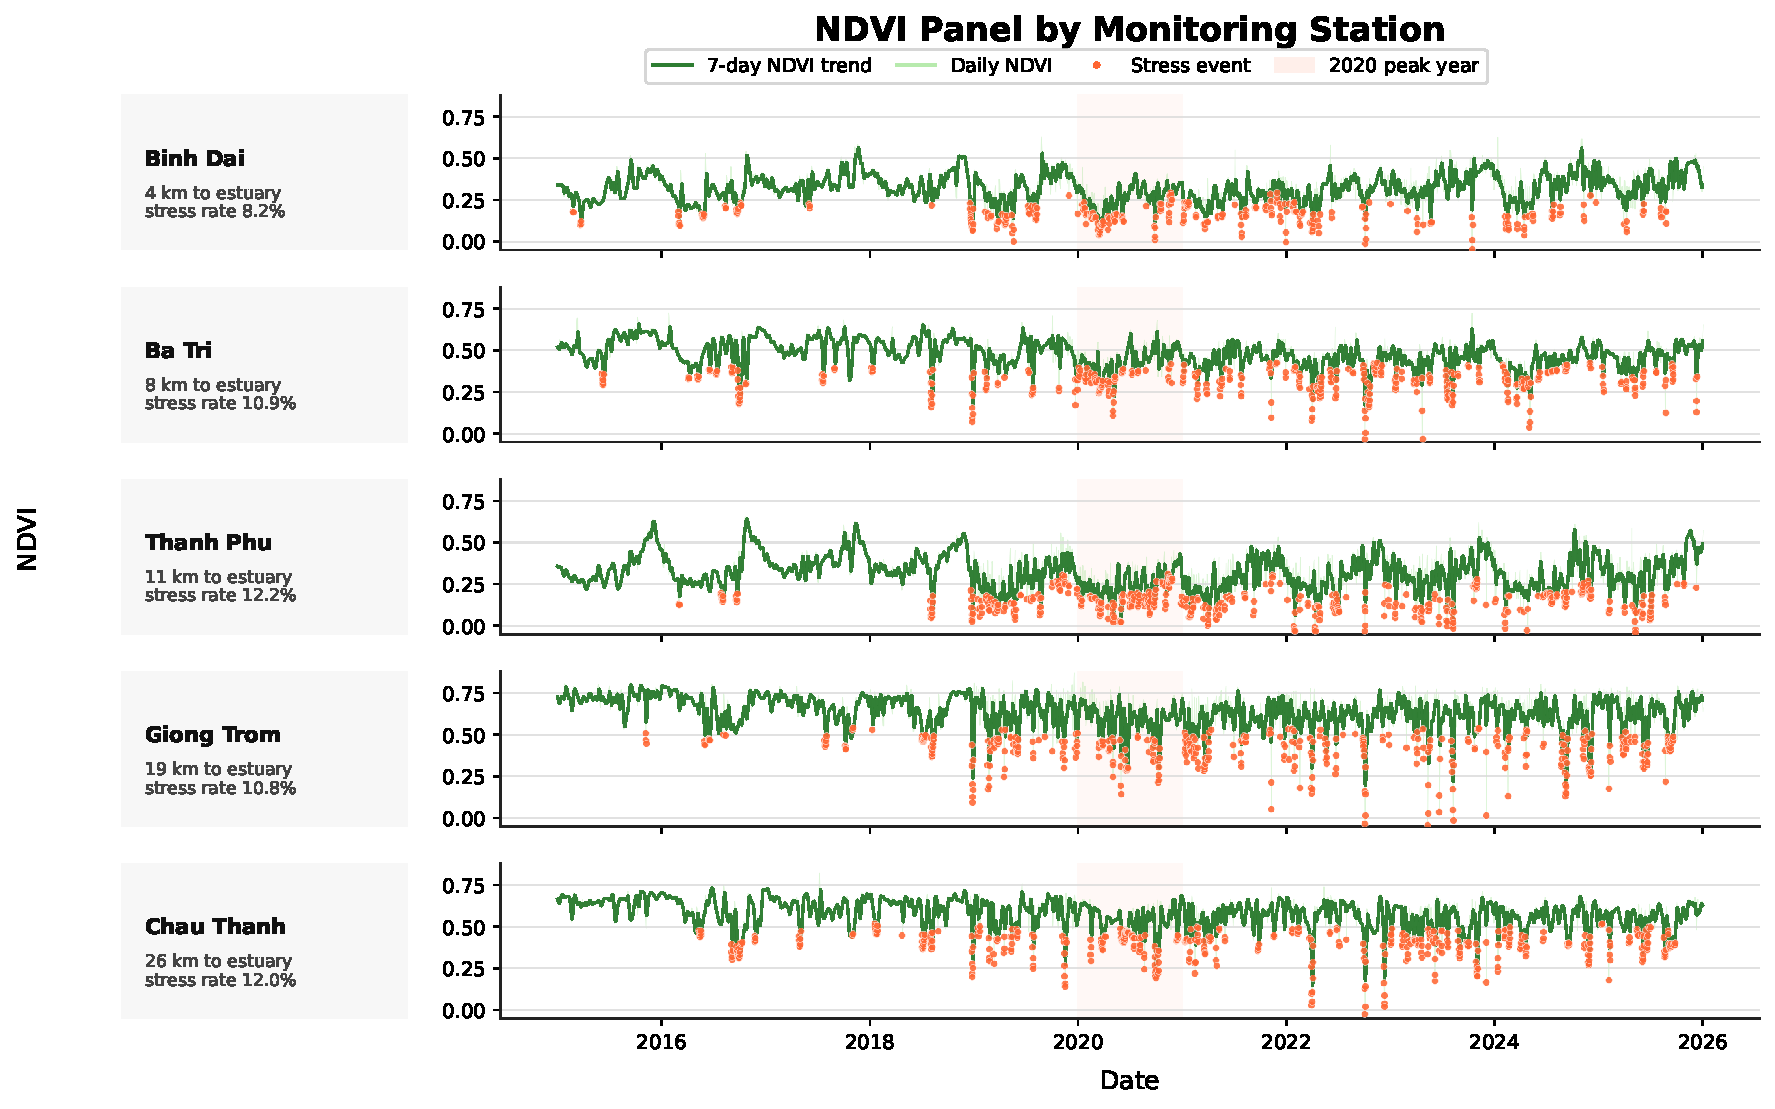
\includegraphics[width=\linewidth]{report_figures/fig2_panel_5_stations.pdf}
        \caption{Five-station NDVI panel}
    \end{subfigure}
    \caption{Two EDA views: vegetation-health dynamics over time and spatial differences across stations.}
    \label{fig:eda}
\end{figure}

\begin{table}[!htbp]
\centering
\caption{Key EDA findings and their implications for modeling}
\label{tab:eda-insights}
\footnotesize
\renewcommand{\arraystretch}{1.05}
\begin{tabularx}{0.98\linewidth}{>{\raggedright\arraybackslash}p{0.25\linewidth}>{\raggedright\arraybackslash}p{0.32\linewidth}>{\raggedright\arraybackslash}X}
\toprule
\textbf{EDA evidence} & \textbf{Interpretation} & \textbf{Modeling implication} \\
\midrule
The year 2020 has the highest stress rate, 21.1\%. & The dataset captures an extreme salinity-drought period, not only average years. & Temporal splitting is necessary; random splitting would produce overly optimistic estimates. \\
Dry-season salinity averages 16.94 PSU versus 7.07 PSU in the wet season, but stress rates remain similar. & Salinity is a background pressure, while the stress label depends on vegetation response and accumulated conditions. & A simple salinity threshold is insufficient; a multivariate model with NDVI, moisture, heat, and rolling features is required. \\
Binh Dai has the highest mean salinity but the lowest stress rate; Chau Thanh is farther from the estuary but has high stress. & Spatial risk is not determined by estuary distance alone. & Geography must be combined with vegetation trends and soil-water conditions. \\
NDVI includes 4,520 direct observations and 15,570 PCHIP/interpolated points. & Satellite data has substantial gaps due to clouds and revisit cycles. & Provenance should be preserved, and interpolation bias should be controlled using \texttt{ndvi\_gap\_days} and \texttt{ndvi\_is\_observed}. \\
\texttt{salinity\_source} is currently \texttt{synthetic\_proxy}. & Salinity is proxy-derived from weather and seasonality, not direct station-level measurement. & This is the main scientific limitation and the first priority for future data improvement. \\
\bottomrule
\end{tabularx}
\renewcommand{\arraystretch}{1.0}
\end{table}

Stress rate varies strongly by year: 2020 has the highest stress rate, consistent with an extreme salinity-drought period. At station level, Thanh Phu and Chau Thanh have higher overall stress rates, while Binh Dai is lower in the processed dataset. This shows that estuary distance is useful but not decisive; the model must also use NDVI tendency, soil moisture, heat, and rainfall history.

A key insight is that crop stress is not equivalent to instantaneous salinity. In the XGBoost feature importance, \texttt{ndvi\_tendency} is the strongest feature, with gain 245.1, much higher than \texttt{salinity\_psu}. Agronomically, this is plausible: crops may tolerate short-term salinity when water status and vegetation vigor remain stable, whereas a persistent decline in NDVI directly indicates loss of crop health.

\section{Preprocessing and Feature Engineering}

\subsection{Cleaning and missing-value treatment}

Satellite observations are not available every day because of cloud cover, revisit cycles, and image-quality filtering. The pipeline aligns each station to a complete daily grid and handles missing values within each station to avoid cross-location leakage. NDVI is sourced from remote-sensing products with different revisit cycles and resolutions, including Sentinel-2 and MODIS vegetation indices \cite{modisvi}. Short gaps up to 14 days are interpolated using PCHIP, edge gaps are filled separately, and \texttt{ndvi\_is\_observed}, \texttt{ndvi\_gap\_days}, and \texttt{ndvi\_interp\_method} are preserved to expose interpolation bias.

During training, columns that are not model inputs or that may create leakage are removed. These include \texttt{date}, source-label columns, target-like variables, \texttt{crop\_stress\_score}, \texttt{ndvi\_zscore}, anomaly flags, and selected salinity/precipitation lag columns that increase multicollinearity without improving interpretability. The remaining feature matrix is imputed with \texttt{ffill().bfill()} within the panel structure and, if missing values remain, median imputation. In the training notebook, this procedure reduces 5,043 missing values to zero after forward/backward filling.

\subsection{Temporal and domain features}

The final XGBoost feature set contains 46 columns grouped as follows:

\begin{itemize}[leftmargin=1.2em, itemsep=1pt]
    \item \textbf{Spatial exposure}: \texttt{lat}, \texttt{lon}, and \texttt{distance\_to\_estuary\_km}.
    \item \textbf{Vegetation condition}: \texttt{ndvi}, \texttt{lst}, \texttt{ndvi\_lag\_1}, \texttt{ndvi\_lag\_3}, \texttt{ndvi\_lag\_7}, and \texttt{ndvi\_tendency}.
    \item \textbf{Meteorology}: temperature, precipitation, ET0, radiation, wind, and 7/15/30-day rolling rainfall features.
    \item \textbf{Soil and salinity}: soil moisture, soil temperature, \texttt{salinity\_psu}, rolling salinity statistics, and salinity tendency.
    \item \textbf{Seasonality}: \texttt{day\_of\_year}, \texttt{month}, \texttt{week}, dry-season flag, \texttt{month\_sin}, and \texttt{month\_cos}.
\end{itemize}

All rolling and lagged features are computed separately by \texttt{location\_id}. This is essential for panel time-series data: each monitoring station is a parallel temporal sequence, so the model must learn shared patterns across locations without allowing one station's future or neighboring history to contaminate another station's feature values.

\section{Modeling Methodology}

\subsection{Temporal split and leakage control}

Because SaltySeq is a forecasting problem, a random split would expose later-year patterns during training and overstate deployment performance. The project uses 2015--2022 for training and 2023--2025 for holdout testing. Within training, \texttt{TimeSeriesSplit} creates five expanding-window folds, where each validation segment follows its corresponding training segment \cite{sklearn-tscv}. The pipeline also verifies no overlap by row index, date, or panel key \texttt{(location\_id, date)}.

Since the positive class represents only 10.8\% of the dataset, the report emphasizes PR-AUC, Recall, and F2-score rather than Accuracy. Precision-recall curves are generally more informative than ROC curves when evaluating classifiers on imbalanced data \cite{saito2015}. In this application, F2-score is especially relevant because missing an actual stress event is usually more costly than issuing a limited number of false alerts.

\subsection{XGBoost backbone}

The main predictive model is XGBoost, a regularized gradient tree boosting system that is well suited for structured tabular data \cite{chen2016xgboost}. Optuna is used for 100 hyperparameter-optimization trials with mean cross-validation AUPRC as the objective \cite{akiba2019optuna}. Class imbalance is handled using \texttt{scale\_pos\_weight = 8.9455}. After tuning, the best model uses 774 trees, maximum depth 4, learning rate 0.0847, subsample 0.928, and column subsample 0.708.

\subsection{Sequential Pattern Mining and GRU}

PrefixSpan mines frequent sequential patterns without generating a large candidate set as in traditional Apriori-style approaches \cite{pei2001prefixspan}. In SaltySeq, each daily record can be discretized into a state such as \texttt{Salt\_High|Soil\_Dry|Temp\_Hot|Rain\_Light}. Patterns are matched using subsequence matching, so a warning can be explained as a sequence of environmental conditions rather than as a single feature value crossing a threshold.

The project also experiments with a PyTorch GRU model using 71 features, including the 46 numeric features and additional PrefixSpan-derived features. GRU is a recurrent neural-network architecture with gating mechanisms for learning sequence dependencies \cite{cho2014gru}. In the current project state, GRU is best interpreted as a deep-learning extension path: it achieves strong recall but produces substantially more false positives than XGBoost.

\section{Experimental Results}

\begin{table}[!htbp]
\centering
\caption{Model comparison on the 2023--2025 holdout test set}
\label{tab:model-results}
\small
\begin{tabular}{lccccc}
\toprule
\textbf{Model} & \textbf{CV AUPRC} & \textbf{Precision} & \textbf{Recall} & \textbf{F1} & \textbf{F2} \\
\midrule
XGBoost & 0.8380 & 0.8740 & 0.9387 & 0.9052 & \textbf{0.9250} \\
Random Forest & 0.7709 & \textbf{0.9175} & 0.7450 & 0.8223 & 0.7741 \\
SVM & 0.7380 & 0.8406 & 0.7137 & 0.7720 & 0.7359 \\
Logistic Regression & 0.7361 & 0.8289 & 0.7179 & 0.7695 & 0.7377 \\
PrefixSpan + GRU & -- & 0.6155 & 0.9302 & 0.7408 & 0.8439 \\
\bottomrule
\end{tabular}
\end{table}

XGBoost achieves the best overall result: test PR-AUC 0.9738, Precision 0.8740, Recall 0.9387, and F2-score 0.9250. Its confusion matrix contains 4,683 true negatives, 95 false positives, 43 false negatives, and 659 true positives. High recall is important because missed stress events can damage production, while Precision 0.8740 shows that false alarms remain controlled.

\begin{figure}[!htbp]
    \centering
    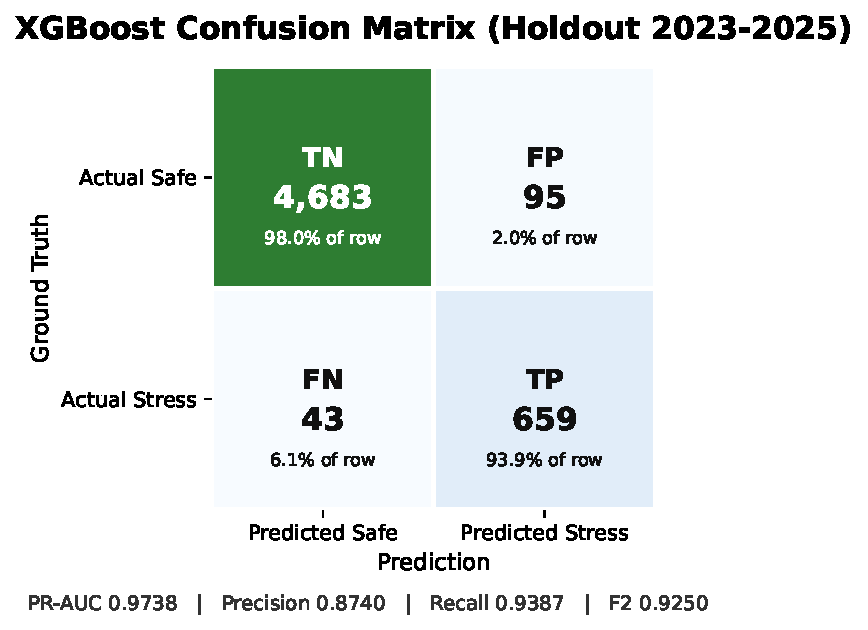
\includegraphics[width=0.52\linewidth]{report_figures/fig4_confusion_matrix.pdf}
    \caption{XGBoost confusion matrix on the 2023--2025 holdout test set.}
    \label{fig:confusion-matrix}
\end{figure}

\begin{figure}[!htbp]
    \centering
    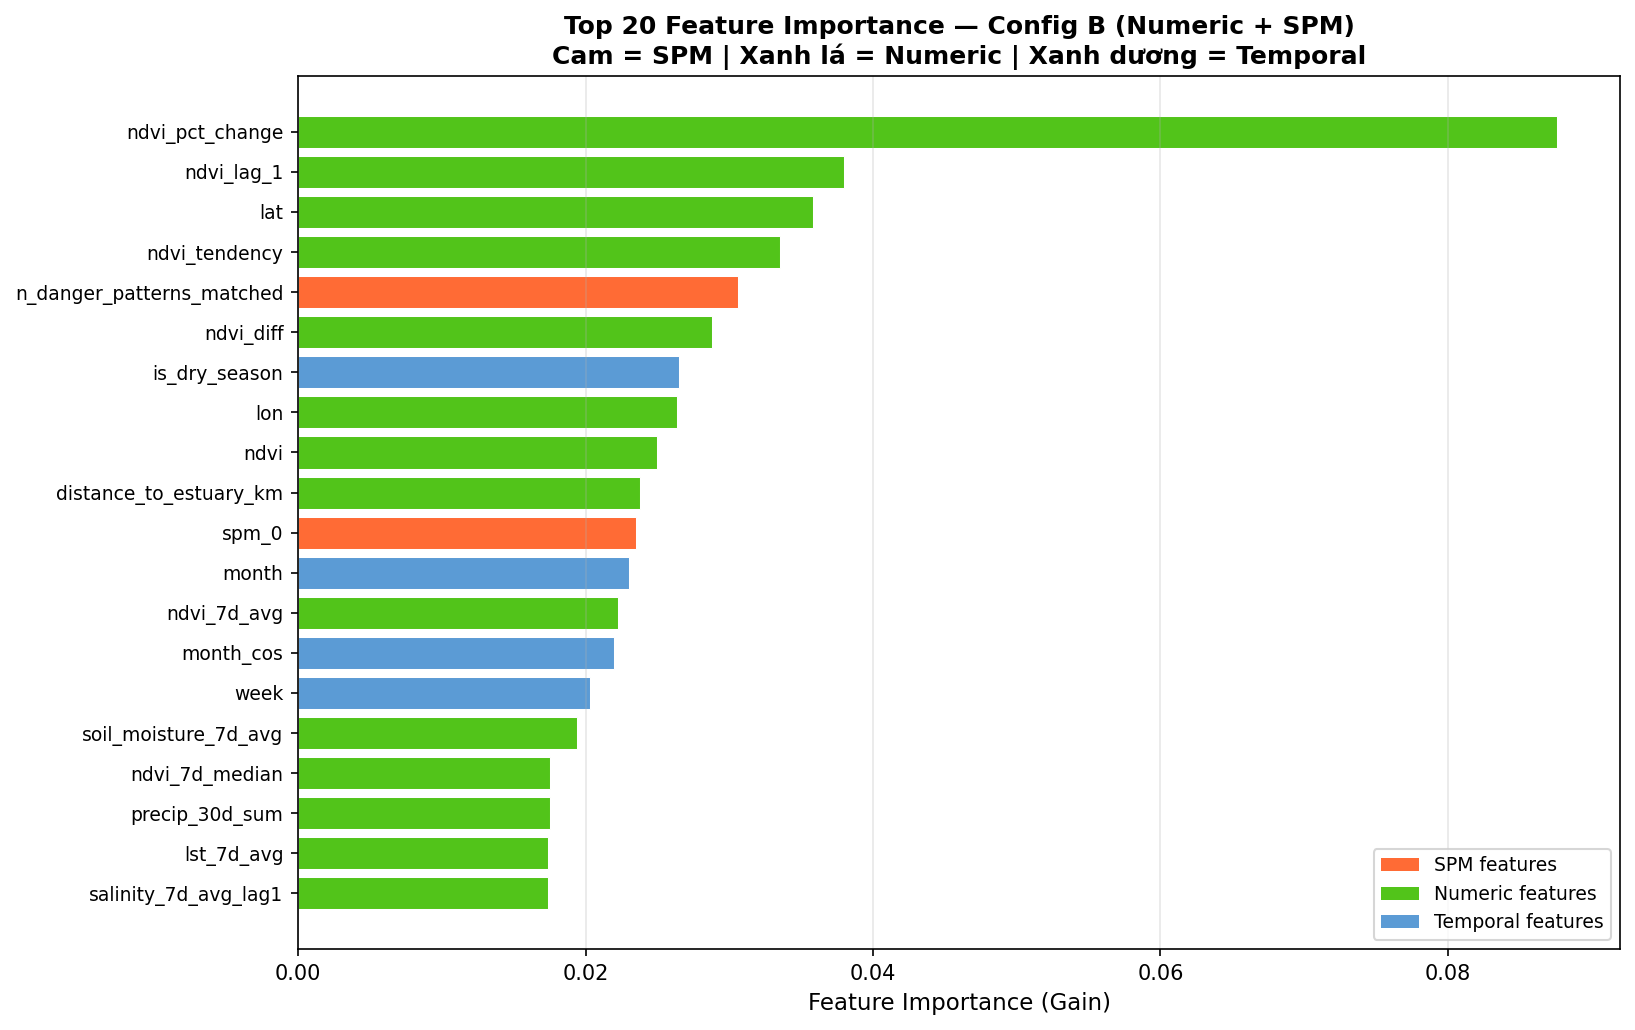
\includegraphics[width=0.72\linewidth]{report_figures/fig3_feature_importance.png}
    \caption{XGBoost feature importance. Vegetation-trend signals such as \texttt{ndvi\_tendency}, \texttt{ndvi}, and \texttt{ndvi\_lag\_1} form the strongest contribution group.}
    \label{fig:feature-importance}
\end{figure}

GRU reaches Recall 0.9302, close to XGBoost, but its Precision is only 0.6155. This means that the recurrent model is sensitive to stress events but triggers many more false positives. Therefore, in the current version, GRU is valuable as a deep-learning extension and comparison point, while XGBoost remains the more reliable backbone for the final system.

\section{Discussion}

The results show that model choice should follow the structure of the data. XGBoost performs strongly because the problem is a feature-rich tabular panel with nonlinear interactions among NDVI, salinity, rainfall, soil moisture, heat, and geography. Logistic Regression and SVM cannot capture these interactions as effectively, while Random Forest has high precision but lower recall. The main defense points are: evaluation uses a real future holdout period; the target is crop-health response rather than a raw salinity threshold; and the SPM layer connects alerts to environmental sequences.

Feature importance provides an agronomically coherent explanation. \texttt{ndvi\_tendency} is the top feature because it measures the direction of vegetation-health change. \texttt{lat}, \texttt{lon}, and \texttt{distance\_to\_estuary\_km} represent the spatial gradient of salinity intrusion. \texttt{lst\_ndvi\_ratio} combines heat pressure with vegetation decline, while \texttt{salinity\_7d\_median} captures sustained salinity instead of a single instantaneous reading.

PrefixSpan contributes interpretability. A sequence such as \texttt{Salt\_High -> Soil\_Dry -> Plant\_DANGER} is easier to communicate than a 46-dimensional vector. However, SPM should not be overstated as the main predictive model. Its role is to support explanation and sequence-aware feature construction, while XGBoost remains the primary classifier.

The main limitation is that \texttt{salinity\_psu} may be proxy-derived when direct station measurements are unavailable, creating risk of systematic bias. Some unrealistic negative LST outliers also remain in the raw data, so a production pipeline should add stricter domain-range checks. Finally, the exported GRU artifact currently uses a short lookback and does not fully exploit longer sequence context; future experiments should test 7-day and 14-day lookbacks, probability calibration, and a separate validation set.

\section{System Deployment and Conclusion}

SaltySeq is packaged as a local demo with FastAPI, SQLite, and a React frontend served by the backend. The main endpoints provide station metadata, date-based feature pre-fill, stress prediction, prediction-history storage, and pipeline-status monitoring. An APScheduler job runs at 06:00 to simulate refresh by writing logs and a status file. The Mekong Sentinel interface includes a station map, feature form, probability gauge, SPM pattern cards, and prediction history.

In conclusion, SaltySeq satisfies the requirements of a complete data-mining project: multi-source ingestion, panel time-series construction, EDA, leakage control, strong tabular modeling, imbalance-aware evaluation, and interactive deployment. XGBoost achieves F2-score 0.9250 on the future holdout set. Next priorities are direct salinity measurement, stricter outlier handling, probability calibration, and stronger temporal models with longer lookback windows.

\footnotesize
\begin{thebibliography}{11}
\setlength{\itemsep}{0pt}
\setlength{\parsep}{0pt}

\bibitem{crispdm}
P. Chapman, J. Clinton, R. Kerber, T. Khabaza, T. Reinartz, C. Shearer, and R. Wirth.
\textit{CRISP-DM 1.0: Step-by-step data mining guide}. SPSS Inc., 2000.
Available: \url{https://www.dataprix.com/files/CRISP-DM.pdf}. Accessed: 15 May 2026.

\bibitem{gorelick2017gee}
N. Gorelick, M. Hancher, M. Dixon, S. Ilyushchenko, D. Thau, and R. Moore.
``Google Earth Engine: Planetary-scale geospatial analysis for everyone.''
\textit{Remote Sensing of Environment}, vol. 202, pp. 18--27, 2017.
doi: 10.1016/j.rse.2017.06.031.

\bibitem{sklearn-tscv}
Scikit-learn developers.
\textit{TimeSeriesSplit documentation}.
Available: \url{https://scikit-learn.org/stable/modules/generated/sklearn.model_selection.TimeSeriesSplit.html}. Accessed: 15 May 2026.

\bibitem{openmeteo}
Open-Meteo.
\textit{Historical Weather API documentation}.
Available: \url{https://open-meteo.com/en/docs/historical-weather-api}. Accessed: 15 May 2026.

\bibitem{copernicusmarine}
Copernicus Marine Service.
\textit{Copernicus Marine APIs and data access documentation}.
Available: \url{https://help.marine.copernicus.eu/en/articles/4794731-which-apis-are-provided}. Accessed: 15 May 2026.

\bibitem{modisvi}
NASA MODIS Land Team.
\textit{MODIS Vegetation Index User's Guide}.
Available: \url{https://modis-land.gsfc.nasa.gov/pdf/MOD13_User_Guide_V61.pdf}. Accessed: 15 May 2026.

\bibitem{saito2015}
T. Saito and M. Rehmsmeier.
``The Precision-Recall Plot Is More Informative than the ROC Plot When Evaluating Binary Classifiers on Imbalanced Datasets.''
\textit{PLOS ONE}, vol. 10, no. 3, e0118432, 2015.
doi: 10.1371/journal.pone.0118432.

\bibitem{chen2016xgboost}
T. Chen and C. Guestrin.
``XGBoost: A Scalable Tree Boosting System.''
In \textit{Proceedings of the 22nd ACM SIGKDD International Conference on Knowledge Discovery and Data Mining}, pp. 785--794, 2016.
Available: \url{https://arxiv.org/abs/1603.02754}.

\bibitem{akiba2019optuna}
T. Akiba, S. Sano, T. Yanase, T. Ohta, and M. Koyama.
``Optuna: A Next-generation Hyperparameter Optimization Framework.''
In \textit{Proceedings of the 25th ACM SIGKDD International Conference on Knowledge Discovery and Data Mining}, pp. 2623--2631, 2019.
Available: \url{https://arxiv.org/abs/1907.10902}.

\bibitem{pei2001prefixspan}
J. Pei, J. Han, B. Mortazavi-Asl, H. Pinto, Q. Chen, U. Dayal, and M.-C. Hsu.
``PrefixSpan: Mining Sequential Patterns Efficiently by Prefix-Projected Pattern Growth.''
In \textit{Proceedings of the 17th International Conference on Data Engineering}, pp. 215--224, 2001.
Available: \url{https://experts.illinois.edu/en/publications/prefixspan-mining-sequential-patterns-efficiently-by-prefix-proje}.

\bibitem{cho2014gru}
K. Cho, B. van Merrienboer, C. Gulcehre, D. Bahdanau, F. Bougares, H. Schwenk, and Y. Bengio.
``Learning Phrase Representations using RNN Encoder--Decoder for Statistical Machine Translation.''
In \textit{Proceedings of EMNLP}, pp. 1724--1734, 2014.
Available: \url{https://aclanthology.org/D14-1179/}.

\end{thebibliography}

\end{document}
